% !TeX encoding = UTF-8
% !TeX spellcheck = it_IT
% !TeX root = formulario.tex

\chapter{Disequazioni di secondo grado}
\section{Definizione}
Una disequazione di secondo grado è una delle seguenti espressione
\begin{equation}
ax^2+bx+c\quad\begin{cases}
>0\\
\geq 0\\
<0\\
\leq 0
\end{cases}\quad a\neq 0
\end{equation}\index{Disequazioni!secondo grado!definizione}
\section{Risoluzione disequazione secondo grado}
\begin{enumerate}
	\item Risolvo l'equazione associata $ax^2+bx+c=0$ (trinomio)
	\item In base alle soluzioni dell'equazione e al delta costruisco il grafico
	\item Leggendo il  grafico risolvo la disequazione
\end{enumerate}\index{Disequazioni!secondo grado!risoluzione}
\section{Trinomio di secondo grado}
\begin{align}
\rosso{a}x^2+\verde{b}x+\blu{c}=&0\quad \rosso{a}\neq 0\\
x_{1,2}=&\dfrac{-\verde{b}\pm\sqrt{\verde{b}^2-4\rosso{a}\blu{c}}}{2\rosso{a}}\\
\Delta=&\verde{b}^2-4\rosso{a}\blu{c}
\end{align}\index{Disequazioni!secondo grado}\index{Delta}\index{Discriminante}
\section{Delta classificazione soluzioni}
\begin{equation}
\rosso{a}x^2+\verde{b}x+\blu{c}=0\quad \rosso{a}\neq 0\quad\begin{cases}
\text{Se $\Delta >0$ Soluzioni distinte}\\
\text{Se $\Delta =0$ Soluzioni coincidenti}\\
\text{Se $\Delta <0$ Nessuna soluzione reale}\\
\end{cases}
\end{equation}\index{Discriminante}\index{Delta}
%\begin{table}
\section{Segno del trinomio delta maggiore di zero}{\textDelta maggiore di zero}
\begin{center}\index{Disequazioni!secondo grado!segno trinomio}
		\begin{tikzpicture}
	\tkzTabInit[color,lgt=5,espcl=3]%
	{$x$ / .8,$\Delta>0$\\ Il segno di\\ $ax^2+bx+c$ /2}%
	{$-\infty$,$x_1$,$x_2$,$+\infty$}%
	\tkzTabLine{ , \genfrac{}{}{0pt}{0}{\text{segno di}}{a}, z
		, \genfrac{}{}{0pt}{0}{\text{segno}}{\text{opposto di}\ a}, z
		, \genfrac{}{}{0pt}{0}{\text{segno di}}{a}, }
	\end{tikzpicture}
	\captionof{figure}{Regola del DICE}
\end{center}\index{Delta}\index{Discriminante}
\section{Segno del trinomio delta uguale a zero}{\textDelta uguale a zero}
\begin{center}
		\begin{tikzpicture}
	\tkzTabInit[color,lgt=5,espcl=3]%
	{$x$ / .8, $\Delta=0$\\ Il segno di\\ $ax^2+bx+c$ / 2}%
	{$-\infty$,$x_1$,$+\infty$}%
	\tkzTabLine{ , \genfrac{}{}{0pt}{0}{\text{segno di}}{ a} , z
		, \genfrac{}{}{0pt}{0}{\text{segno di}}{a}, }
	\end{tikzpicture}
	\captionof{figure}{Regola Segue a}
\end{center}
\section{Segno del trinomio delta minore di zero}{\textDelta minore di zero}
\begin{center}
		\begin{tikzpicture}
	\tkzTabInit[color,lgt=5,espcl=5]%
	{$x$/.8,$\Delta<0$\\ Il segno di\\ $ax^2+bx+c$/2}%
	{$-\infty$,$+\infty$}%
	\tkzTabLine{ , \genfrac{}{}{0pt}{0}{\text{segno di}}{ a}, }
	\end{tikzpicture}
	\captionof{figure}{Regola  Solo a}
\end{center}\index{Delta}\index{Discriminante}
